\chapter{刚体力学基础 \quad 动量矩}

\begin{introduction}
	\item \nameref{5.1}
	\item \nameref{5.2}
	\item \nameref{5.3}
	\item \nameref{5.4}
	\item \nameref{5.5}
\end{introduction}

\section{刚体的基本运动} \label{5.1}

\subsection{刚体}

\begin{definition}[刚体] \label{C5-df1}
	{\heiti 刚体} 在力作用下, 大小和形状都保持不变的物体. 在力作用下, 组成刚体的所有质点之间的距离始终保持不变. 
\end{definition}

\subsection{刚体的平动}

刚体运动时, 若\textbf{在刚体内所作的任意一条直线都始终保持和自身平行}, 这种运动就称为刚体的平行移动, 简称刚体的平动. 

如下图, $AB$杆的运动即为刚体平动: 

\begin{figure}[htbp]
	\centering
	\includegraphics[scale=0.8]{C5-kbfig5.2.eps}
	\caption{课本P84 图5.2}
\end{figure}

\textbf{在任意时刻, 平动刚体上各点的速度加速度都相同. }

\subsection{刚体的定轴转动}

如果\textbf{转动刚体的转轴相对参考系是固定不动的}, 这时刚体的转动就称为刚体绕定轴转动. 

刚体的角坐标$\theta$是时间的单值函数

\begin{equation}
	\theta = f(t) \label{C5-eq1}
\end{equation}

刚体在时刻$t$的角速度$\omega$是刚体角坐标对时间的一阶导数

\begin{equation}
	\omega = \lim\limits_{\Delta t \to 0} \dfrac{\Delta \theta}{\Delta t} = \dv{\theta}{t} = f'(t) \label{C5-eq2}
\end{equation}

每分钟转过的圈数$n$ (简称转速), 和角速度的关系

\begin{equation}
	\omega = \dfrac{\pi n}{30} \label{C5-eq3}
\end{equation}

角速度$\omega$对时间的一阶导数就是绕定轴转动刚体的角加速度$\alpha$

\begin{equation}
	\alpha = \lim\limits_{\Delta t \to 0} \dfrac{\Delta \omega}{\Delta t} = \dv{\omega}{t} = \dv[2]{\theta}{t} = f''(t) \label{C5-eq4}
\end{equation}

\section{刚体绕定轴转动微分方程} \label{5.2}

\subsection{力矩}

\begin{definition}[力矩] \label{C5-df2}
	{\heiti 力对转轴$z$之矩} 力$\va*{F}$的大小与$O$点到$\va*{F}$的作用线间垂直距离$h$(即力臂)的乘积. 任意力$\va*{F}$对轴z之矩就等于$\va*{F}_{\perp}$对轴$z$之矩. 
	
	\begin{equation}
		M_z (\va*{F}) = M_z (\va*{F}_{\perp}) = \pm Fh = \pm F_{\perp} h = \pm Fr\sin \varphi = 2 S_{\triangle OAB} \label{C5-eq5}
	\end{equation}
	
	当力平行于轴或通过轴时, 力对该轴之矩皆为零. 
	
	{\heiti 力对点$O$之矩} 矢径$\va*{r}$与力$\va*{F}$的叉积. 
	
	\begin{equation}
		\va*{M}_O = \va*{r} \times \va*{F} \label{C5-eq6}
	\end{equation}
	
	其大小为
	
	\begin{equation}
		\abs{\va*{M}_O} = Fr\sin \alpha = 2S_{\triangle OAB} \label{C5-eq7}
	\end{equation}
	
\end{definition}

\begin{figure}[htbp]
	\centering
	\begin{minipage}[t]{0.48\textwidth}
		\centering
		\includegraphics[scale=1.2]{C5-kbfig5.6.eps}
		\label{C5-kbfig5.6}
	\end{minipage}
	\begin{minipage}[t]{0.48\textwidth}
		\centering
		\includegraphics[scale=1.2]{C5-kbfig5.7.eps}
		\label{C5-kbfig5.7}
	\end{minipage}
\end{figure}

\subsection{刚体绕定轴转动微分方程}

\begin{equation}
	J_z \dv{\omega}{t} = M_z \label{C5-eq8}
\end{equation}

其中, $J_z$为刚体对$z$轴的转动惯量. 

式(\ref{C5-eq8})即为刚体绕定轴转动微分方程, 也称转动定律. 它表明, 刚体绕定轴转动时, \textbf{刚体对该轴的转动惯量与角加速度的乘积等于作用在刚体上所有外力对该轴之矩的代数和. }

\subsection{转动惯量} \label{5.2.3}

刚体对$z$轴的转动惯量为

\begin{equation}
	J_z = \sum\limits_{k} \Delta m_k r_k^2 \label{C5-eq9}
\end{equation}

特别地, 对于质量连续分布的刚体

\begin{equation}
	J_z = \int_{V} r^2 \dd{m} \label{C5-eq10}
\end{equation}

\textbf{常见刚体的转动惯量见附表(\ref{A1-tb1}).} 

\vskip 0.3cm

下面介绍两个重要的定理. 

\begin{theorem}[平行轴定理] \label{C5-th1}
	
	刚体对任意已知轴的转动惯量, 等于刚体对通过质心并与该已知轴平行的轴的转动惯量加上刚体质量与两轴间垂直距离$h$平方的乘积. 
	
	\begin{equation}
		J_z = J_c + md^2 \label{C5-eq11}
	\end{equation}
	
	其中, $J_z$为刚体绕任意轴的转动惯量, $J_c$为刚体绕通过质心轴的转动惯量, $d$为两轴间垂直距离. 
	
\end{theorem}

\begin{theorem}[(薄板)垂直轴定理] \label{C5-th2}
	
	\begin{equation}
		J_z = J_x + J_y \label{C5-eq12}
	\end{equation}
	
	$x$, $y$轴在薄板内, $z$轴垂直薄板. 
	
\end{theorem}

薄板垂直轴定理示意图如下: 

\begin{figure}[htbp]
	\centering
	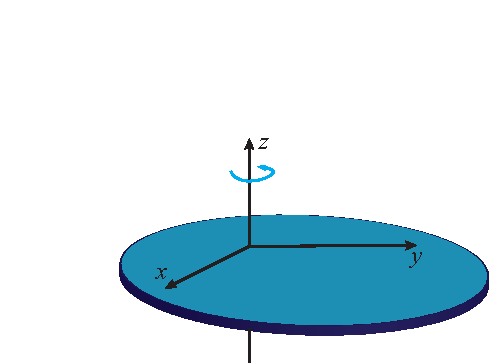
\includegraphics[scale=1.2]{C5-fig1.pdf}
	\caption{薄板垂直轴定理示意图}
	\label{C5-fig1}
\end{figure}

\section{绕定轴转动刚体的动能 \quad 动能定理} \label{5.3}

\begin{enumerate}
	
	\item 绕定轴转动刚体的动能
	
	\begin{equation}
		E = \dfrac{1}{2} J_z \omega^2 \label{C5-eq13}
	\end{equation}
	
	\item 力矩的功
	
	\begin{equation}
		A = \int_{\theta_1}^{\theta_2} M_z(\va*{F}) \dd{\theta} \label{C5-eq14}
	\end{equation}
	
	\item 绕定轴转动刚体的动能定理
	
	\begin{equation}
		\dd{\qty(\dfrac{1}{2} J_z \omega^2)} = \dd{A} \Longrightarrow \dfrac{1}{2} J_z \omega_2^2 - \dfrac{1}{2} J_z \omega_1^2 = A \label{C5-eq15}
	\end{equation}
	
\end{enumerate}

\newpage

\section{动量矩和动量矩守恒定律} \label{5.4}

\subsection{动量矩(角动量)}

\begin{definition}[动量矩(角动量)] \label{C5-df3}
	
	质点动量对$O$点之矩定义为位矢$\va*{r}$和动量$m\va*{v}$的叉积, 即
	
	\begin{equation}
		\va*{L}_O = \va*{r} \times m \va*{v} \label{C5-eq16}
	\end{equation}
	
	刚体对$z$轴的动量矩
	
	\begin{equation}
		L_z = J_z \omega \label{C5-eq17}
	\end{equation}
	
\end{definition}

\subsection{质点动量矩定理和动量矩守恒定律}

\begin{theorem}[质点动量矩定理] \label{C5-th3}
	在惯性系中, 质点对任意固定点$O$的动量矩对时间的导数, 等于作用在质点上所有力的合力对同一点$O$之矩. 
	
	\begin{equation}
		\dv{\va*{L}_O}{t} = \va*{r} \times \va*{F} = \va*{M}_O \label{C5-eq18}
	\end{equation}

\end{theorem}

\begin{axiom}[质点动量矩守恒定律] \label{C5-ax1}
	
	当作用在质点上的合力对固定点之矩总是为0时, 质点动量对该点的矩为常矢量. 
	
	\begin{equation}
		\va*{M}_O = 0 \Longrightarrow \va*{L}_O = \overrightarrow{\text{Const}} \label{C5-eq19}
	\end{equation}
		
\end{axiom}

\textbf{质点在有心力作用下的运动过程中, 质点对力心的动量矩守恒. }

\subsection{刚体绕定轴转动情况下的动量矩定理和动量矩守恒定律}

\begin{theorem}[刚体绕定轴转动情况下的动量矩定理] \label{C5-th4}
	\begin{equation}
		\dv{t}(J_z\omega) = M_z \label{C5-eq20}
	\end{equation}
	
	上式表明, 绕定轴转动刚体动量矩对时间的导数, 等于作用在刚体上所有外力对转轴之矩的代数和. 
	
	对式(\ref{C5-eq20})积分, 得
	
	\begin{equation}
		{(J_z\omega)}_t - {(J_z\omega)}_{t_0} = \int_{t_0}^{t} M_z \dd{t} \label{C5-eq21}
	\end{equation}

    上式表明, 定轴转动刚体的动量矩在某一时间间隔内的增量, 等于同一时间间隔内作用在刚体上的冲量矩. 
    
\end{theorem}

类似定律\ref{C5-ax1}, 有

\begin{equation}
	M_z = 0 \Longrightarrow J_z \omega = \overrightarrow{\text{Const}} \label{C5-eq22}
\end{equation}

\section{第4次作业部分题目归纳} \label{5.5}

\subsection{转动惯量的计算}

\begin{enumerate}
	
	\item (作业T5) 一块质量分布均匀的等边三角形薄板, 质量为$m$, 边长为$a$, 则它相对于通过其一边的轴的转动惯量为 \uline{$ma^2/8$}. 
	
\end{enumerate}

\subsection{圆盘(滑轮)}

\begin{enumerate}
	
	\item (作业T22) 一具有光滑转轴的定滑轮, 半径为$R$, 质量为$m/4$, 质量均匀分布在滑轮的边缘上, 从而对转轴的转动惯量为$J = mR^2/4$. 一轻绳跨过该定滑轮, 轻绳与滑轮间无相对滑动, 其左端有一质量为$m$的人爬在轻绳上, 而右端则系了一质量为$m/2$的重物, 如图(\ref{C5-fig2})所示. 当人从静止开始相对于轻绳匀速向上攀爬时, 求重物上升的加速度. 
	
\end{enumerate}

\begin{figure}[htbp]
	\centering
	\begin{minipage}[t]{0.48\textwidth}
		\centering
		\includegraphics[scale=0.6]{C5-fig2.eps}
		\caption{作业T22题图}
		\label{C5-fig2}
	\end{minipage}
	\begin{minipage}[t]{0.48\textwidth}
		\centering
		\includegraphics[scale=0.9]{C5-fig3.eps}
		\caption{作业T15题图}
		\label{C5-fig3}
	\end{minipage}
\end{figure}

\subsection{杆}

\begin{enumerate}
	
	\item (作业T15) 如图(\ref{C5-fig3})所示, 长为$l$, 质量为$M$的匀质直杆可绕过其一端$O$的水平位置无初速释放, 当转动到与水平方向成$30^{\circ}$时, 有一质量为$m = M/3$的子弹以水平速度$v_0$射入直杆的下端点并马上嵌在杆中不动, 则子弹射入后瞬间杆的角速度 \uline{$\omega = \sqrt{3g/8l} + v_0/4l$}.
	
\end{enumerate}
